\chapter{黏性流动}\label{ch:b2:viscous-flows}

倒出一罐蜂蜜，它便缓慢而黏稠地流成一道细带；倒出一罐
水，则很快流尽。用勺子分别在两者中搅动：蜂蜜始终阻挡着勺子，
无论速度多快；水在你快速搅动之前几乎毫无反应，
一旦快起来，便会打转。二者的差别在于\emph{动力黏度}——
即流体的内摩擦——以及动力黏度与惯性之间的较量，
这一较量可用一个数概括，即雷诺数，
它决定流动是有序分层地缓慢流动，还是翻滚成湍流。本章在欧拉方程中加入黏性力，
求解工程师常用的两类层流，
并解释为何在高雷诺数下，
动力黏度只集中于壁面附近的薄层之中，
却仍使每一辆汽车、每一艘船和每一架飞机耗费大部分燃料。

\begin{omfigure}
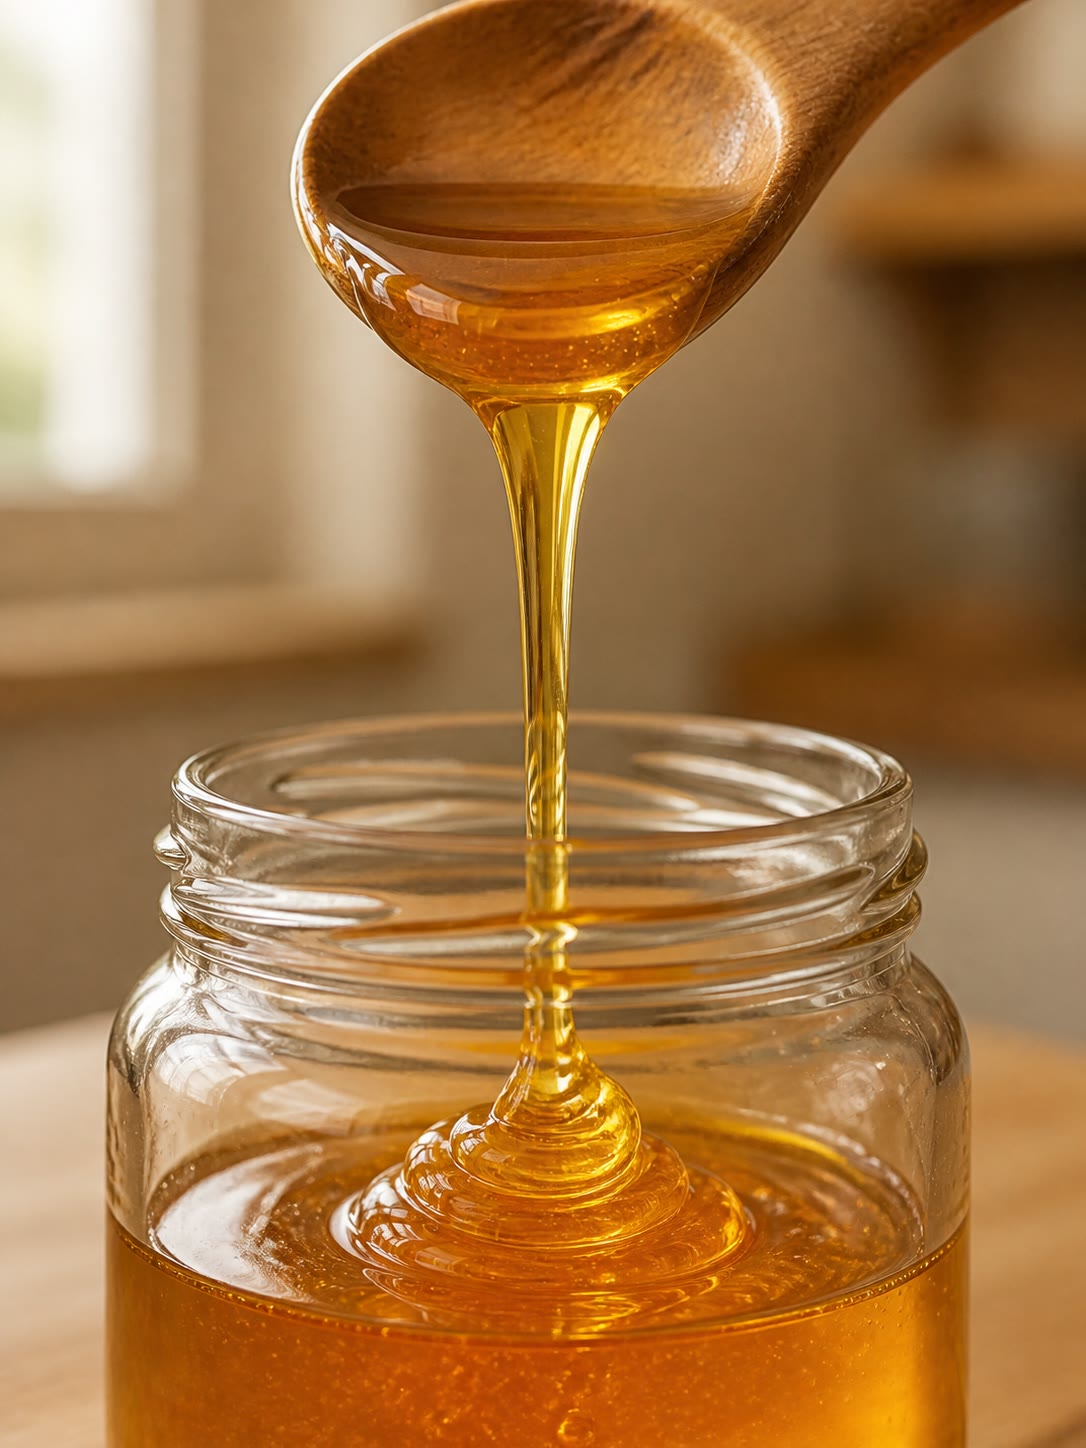
\includegraphics[width=0.34\linewidth]{images/book4/ai/b4-04-honey-spoon-viscous.jpg}

{\small 蜂蜜以细而稳定的细带流下，落地时卷曲：动力黏度是水的一万倍，使惯性可以忽略——即蠕动流。}
\end{omfigure}


\section{动力黏度与纳维–斯托克斯方程}

\begin{definition}[牛顿黏性]\label{def:b2:viscous-flows:viscosity}
\index{黏度}\index{动力黏度}\index{运动黏度}\index{切应力}\index{牛顿流体}
在平面剪切流 $\vect v = v_x(y)\,\vect e_x$ 中，
位于 $y = $ 常数面上方的流体（通过面元
$\dd S$）施加于其下方流体的切向力
\[
\dd\vect F = \eta\,\frac{\dd v_x}{\dd y}\,\dd S\;\vect e_x ,
\]
带动较慢的一层向前，同时自身受到其反向拖拽。
\emph{切应力}为 $\tau = \eta\,\dd v_x/\dd y$；系数
$\eta$（单位 \unit{Pa.s}）为流体的\emph{动力黏度}，
并 $\nu = \eta/\rho$（\unit{m^2/s}）为其\emph{运动黏度}。流体
若 $\eta$ 不随剪切速率变化，则称为\emph{牛顿流体}：
水、空气、油类、酒精属于此类；血液、涂料、番茄酱和聚合物熔体
则不是。在 \qty{20}{\degreeCelsius} 下的数量级：空气 $\eta =
\qty{1.8e-5}{Pa.s}$（$\nu = \qty{1.5e-5}{m^2/s}$），水 $\qty{1.0e-3}{Pa.s}$
（$\nu = \qty{1.0e-6}{m^2/s}$），橄榄油 $\qty{0.08}{Pa.s}$，甘油
$\qty{1.5}{Pa.s}$，蜂蜜 $\sim\qty{10}{Pa.s}$。液体
受热时变稀，气体则变稠。
\end{definition}

\begin{proposition}[黏性力密度；无滑移条件]\label{prop:b2:viscous-flows:density}
\index{无滑移条件}\index{黏性力密度}
在平面剪切流中，位于 $y$ 与 $y + \dd y$ 之间的流体薄层所受的
净黏性力，按单位体积计为 $\eta\,\dd^2v_x/\dd y^2$：
动力黏度作为体积力密度 $\eta\,\Delta\vect v$ 起作用（其中
拉普拉斯算子按分量逐一作用），这一结论对任意
不可压缩流动都成立。在固体壁面处流体\emph{附着}于壁面，其速度与壁面速度相等（即
\emph{无滑移条件}）；这正是风扇叶片上会积尘的原因，
也是壁面受到黏性阻力的原因。
\end{proposition}

\begin{proof}
薄层上方施加的拉力为 $\eta\,v_x'(y + \dd y)\dd S$，下方施加的为
$-\eta\,v_x'(y)\dd S$，合力为 $\eta v_x''\,\dd y\,\dd S$。一般
形式在本阶段不加证明地承认（它可由把应力写成速度梯度的
对称线性函数得到）。无滑移条件
是实验结论。
\end{proof}

\begin{theorem}[纳维–斯托克斯方程]\label{thm:b2:viscous-flows:ns}
\index{纳维–斯托克斯方程}
不可压缩的牛顿流体满足
\[
\rho\Bigl(\frac{\partial\vect v}{\partial t} + (\vect v\cdot\operatorname{\vect{grad}})
\vect v\Bigr) = -\operatorname{\vect{grad}}P + \rho\vect g + \eta\,\Delta\vect v ,
\qquad \operatorname{div}\vect v = 0 ,
\]
在每个壁面上均满足无滑移条件。欧拉方程是
$\eta = 0$ 时的情形。
\end{theorem}
\admitted

\begin{omfigure}
\begin{tikzpicture}[font=\small, x=1cm, y=1cm, >=Stealth]
  \begin{scope}
    \draw[thick] (-0.2,0) -- (3.6,0); \fill[pattern=north east lines] (-0.2,-0.18) rectangle (3.6,0);
    \draw[thick, omExo] (-0.2,2.2) -- (3.6,2.2); \fill[pattern=north east lines, pattern color=omExo] (-0.2,2.2) rectangle (3.6,2.38);
    \draw[omExo, very thick, ->] (1.4,2.6) -- (2.6,2.6) node[right, font=\footnotesize] {$U$};
    \foreach \y in {0.4,0.8,...,2.0} \draw[omDef, thick, ->] (0.4,\y) -- ({0.4+1.1*\y/2.2*1.8},\y);
    \draw[omDef, thick] (0.4,0) -- (2.2,2.2);
    \node[font=\footnotesize] at (1.8,-0.5) {库埃特流：$v_x = Uy/h$，$\tau = \eta U/h$};
    \draw[<->] (3.3,0) -- (3.3,2.2) node[midway, right, font=\footnotesize] {$h$};
  \end{scope}
  \begin{scope}[xshift=7.2cm]
    \draw[thick, fill=omDef!10] (0,0.6) rectangle (3.0,1.6);
    \draw[omThm, very thick, ->] (1.5,1.6) -- (2.6,1.6) node[above, font=\footnotesize] {$\eta v_x'(y+\dd y)\,\dd S$};
    \draw[omThm, very thick, ->] (1.5,0.6) -- (0.4,0.6) node[below, font=\footnotesize] {$\eta v_x'(y)\,\dd S$};
    \node[font=\footnotesize] at (-0.5,1.6) {$y + \dd y$};
    \node[font=\footnotesize] at (-0.4,0.6) {$y$};
    \node[font=\footnotesize] at (1.5,-0.5) {净：$\eta\,v_x''\,\dd y\,\dd S$};
  \end{scope}
\end{tikzpicture}

{\small 左图：固定平板与
以 $U$ 运动的平板之间的平面库埃特流——速度线性分布，各层剪切应力相同。
右图：流体薄层所受的黏性力；它们相互抵消，
除非速度分布是弯曲的。}
\end{omfigure}

\begin{example}[桌面上的切应力]\label{ex:b2:viscous-flows:table}
一层厚 \qty{0.1}{mm} 的油膜（$\eta = \qty{0.1}{Pa.s}$）夹在平板与
桌面之间，平板以 \qty{1}{m/s} 滑动：$\tau = \eta U/h = \qty{1}{kPa}$，
相当于作用在十分之一平方米上的 \qty{100}{N} 力——即润滑轴承的原理，
此处黏性阻力取代了干摩擦，而干摩擦力要大
一百倍。一勺蜂蜜，\qty{10}{Pa.s}，厚 \qty{1}{mm}，
以 \qty{1}{mm/s} 的速度下流：$\tau = \qty{10}{Pa}$，恰好等于
单位面积上一毫米厚蜂蜜的重力——这正是它以该速度下流的原因。
\end{example}

\section{雷诺数}

\begin{definition}[雷诺数]\label{def:b2:viscous-flows:reynolds}
\index{雷诺数}\index{层流}\index{湍流}
对于特征速率为 $U$、特征长度为 $L$ 的流动，称
\emph{雷诺数}
\[
\mathrm{Re} = \frac{\rho UL}{\eta} = \frac{UL}{\nu}
\]
为惯性项
$\rho(\vect v\cdot\operatorname{\vect{grad}})\vect v \sim \rho U^2/L$ 与
黏性项 $\eta\Delta\vect v \sim \eta U/L^2$ 在纳维–斯托克斯
方程中的数量级之比。当 $\mathrm{Re} \ll 1$ 时惯性可忽略，流动为
\emph{蠕动流}（黏性、可逆、平滑）；当 $\mathrm{Re} \gg 1$
黏性仅在壁面附近不可忽略，流动为
理想流体的流动——直到超过量级为 $10^3$ 的阈值（以直径为基准，管道中约为 $2000$
至 $3000$）时，流动变为\emph{湍流}：
非定常、混乱，各尺度上都布满涡旋。二者之间，流动为\emph{层流}：
定常且成层。
\end{definition}

\begin{example}[雷诺数的日常例子]\label{ex:b2:viscous-flows:revalues}
细菌（\qty{1}{\micro m}，\qty{30}{\micro m/s}，水中）：$\mathrm{Re} =
3 \times 10^{-5}$ ——它生活在没有惯性的世界里，停止
其鞭毛一停，它便在一个原子直径内停下。毛细血管中的血液：
$10^{-3}$；下落的尘粒：$10^{-2}$；金鱼：$10^3$；游泳者：
$10^6$；以 \qty{30}{m/s} 行驶的汽车（长 \qty{4}{m}）：$8 \times 10^6$；客机：$10^8$；
墨西哥湾流：$10^{11}$。几何形状与雷诺数均相同的两个流动为
\emph{相似}的：正是由此，\qty{1}{m} 的
船模可在拖曳水池中试验，飞机模型则可在风洞中试验。
\end{example}

\section{层流：库埃特、泊肃叶、斯托克斯}

\begin{proposition}[管道中的泊肃叶流动]\label{prop:b2:viscous-flows:poiseuille}
\index{泊肃叶流动}\index{水力阻力}
对于半径为 $R$、长为 $L$ 的水平圆柱形管道，在
两端压强差 $\Delta P = P_1 - P_2$ 的驱动下，定常
层流为
\[
v(r) = \frac{\Delta P}{4\eta L}\,(R^2 - r^2) , \qquad
D_V = \frac{\pi R^4}{8\eta L}\,\Delta P :
\]
速度分布为抛物线形，在轴线上最大，平均速率
$\langle v\rangle = v_{\max}/2$。流量与
压降成正比（泊肃叶定律），比例系数为\emph{水力阻力}
$R_h = \Delta P/D_V = 8\eta L/\pi R^4$，流量还与半径的
\emph{四次方}成正比。壁面切应力为 $\tau_w = \Delta P\,R/2L = 4\eta\langle v
\rangle/R$。适用条件为 $\mathrm{Re} = 2R\langle v\rangle/\nu \lesssim 2000$。
\end{proposition}

\begin{proof}
定常，$\vect v = v(r)\vect e_z$（故对流项为零：$\vect v
\cdot\operatorname{\vect{grad}}$ 只沿 $z$ 方向作用，而沿该方向
无变化）。沿 $z$ 方向的纳维–斯托克斯方程为 $0 = -\partial_zP + \eta\Delta v$，而
沿径向 $\partial_rP = 0$：$P$ 仅依赖于 $z$，$\Delta v$ 仅依赖于 $r$，故
两边都等于常数，$\partial_zP = -\Delta P/L$。在柱坐标
坐标下 $\Delta v = \frac1r\frac{\dd}{\dd r}\bigl(r\frac{\dd v}{\dd r}\bigr)$
（此处直接给出；它是圆柱壳层上黏性力的平衡，
即 $2\pi rL\,\eta v'$ 在 $r$ 与 $r + \dd r$ 处的差）。对 $v$ 积分两次，
由轴上速度有限及 $v(R) = 0$，即得抛物线；$D_V = \int_0^Rv\,2\pi
r\,\dd r$。壁面切应力为 $-\eta v'(R)$；等价地，压强
力 $\pi R^2\Delta P$ 与壁面摩擦力 $2\pi RL\tau_w$ 相平衡。
\end{proof}

\begin{omfigure}
\begin{tikzpicture}[font=\small, x=1cm, y=1cm, >=Stealth]
  \begin{scope}
    \draw[thick] (-2.8,1.0) -- (2.8,1.0) (-2.8,-1.0) -- (2.8,-1.0);
    \fill[pattern=north east lines] (-2.8,1.0) rectangle (2.8,1.15); \fill[pattern=north east lines] (-2.8,-1.0) rectangle (2.8,-1.15);
    \draw[omDef, thick, domain=-1:1, samples=40] plot ({-0.9+1.8*(1-\x*\x)},\x);
    \foreach \y in {-0.8,-0.6,...,0.8} \draw[omDef, ->] (-0.9,\y) -- ({-0.9+1.8*(1-\y*\y)-0.05},\y);
    \draw[dashed] (-0.9,-1) -- (-0.9,1);
    \node[omDef, font=\footnotesize] at (1.6,0.3) {$v_{\max}$};
    \node[font=\footnotesize] at (-2.3,0.0) {$P_1$}; \node[font=\footnotesize] at (2.4,0.0) {$P_2$};
    \node[font=\footnotesize] at (0,-1.5) {$v(r) = \dfrac{\Delta P}{4\eta L}(R^2 - r^2)$};
  \end{scope}
  \begin{scope}[xshift=7.6cm]
    \draw[thick] (-2.2,0) -- (2.2,0) (-2.2,0.5) -- (2.2,0.5) (-2.2,-0.5) -- (2.2,-0.5);
    \draw[thick] (-2.2,-0.5) -- (-2.2,0.5) (2.2,-0.5) -- (2.2,0.5);
    \fill[omDef!15] (-2.2,0) rectangle (2.2,0.5);
    \draw[omThm, very thick, ->] (-3.2,0.25) -- (-2.25,0.25) node[pos=0.2, above, font=\footnotesize] {$P_1$};
    \draw[omThm, very thick, ->] (3.2,0.25) -- (2.25,0.25) node[pos=0.2, above, font=\footnotesize] {$P_2$};
    \draw[omProp, very thick, ->] (0.8,0.5) -- (-0.4,0.5) node[above, font=\footnotesize, pos=0.9] {$\tau(r+\dd r)$};
    \draw[omProp, very thick, ->] (-0.4,0.0) -- (0.8,0.0) node[below, font=\footnotesize, pos=0.9] {$\tau(r)$};
    \node[font=\footnotesize] at (0,-1.3) {壳层 $[r, r + \dd r]$：压强 $=$ 黏性阻力};
  \end{scope}
\end{tikzpicture}

{\small 左图：泊肃叶流动——管道中的抛物线形速度分布，
由压降 $P_1 - P_2$ 驱动。右图：受力平衡，
对流体圆柱壳层而言，其两端的压强差
与内外表面上的黏性应力相平衡。}
\end{omfigure}

\begin{example}[四次方]\label{ex:b2:viscous-flows:fourth}
注射针头的内径为 \qty{0.4}{mm}、长为 \qty{3}{cm}，
水，拇指施加的压强为 \qty{20}{kPa}：$D_V = \pi(2 \times 10^{-4})^4 \times 2 \times
10^4/(8 \times 10^{-3} \times 0.03) = \qty{0.42}{mL/s}$；内径加倍的针头
流量为其十六倍。动脉因斑块而使其半径收窄至 $70\%$，
其阻力变为原来的 $(1/0.7)^4 = 4.2$ 倍：人体通过
提高上游压强来补偿，这也是动脉粥样硬化
与高血压常同时出现的原因之一。
\end{example}

\begin{proposition}[斯托克斯阻力]\label{prop:b2:viscous-flows:stokes}
\index{斯托克斯定律}\index{终端速度}\index{沉降}
半径为 $R$ 的球体以速率 $v$ 在流体中运动，其中
$\mathrm{Re} = 2\rho vR/\eta \ll 1$，所受阻力为
\[
F = 6\pi\eta Rv ,
\]
方向与其速度相反。密度为 $\rho_s$ 的球体在密度为 $\rho$ 的流体中下落，
达到\emph{终端速度}，$v_\infty =
\dfrac{2R^2(\rho_s - \rho)g}{9\eta}$——沉降、
离心分离与密立根油滴实验所适用的规律。
\end{proposition}

\begin{proof}
阻力在本阶段不加证明地承认（它是绕球体蠕动流方程的
精确解，其中三分之二为黏性摩擦，三分之一为
压强）。终端速度：重力减去浮力，$\tfrac43\pi R^3(\rho_s -
\rho)g$ 等于阻力；事后须检验 $\mathrm{Re} \ll 1$。
\end{proof}

\begin{example}[雾、雨与尘埃]\label{ex:b2:viscous-flows:fog}
空气中一颗直径为 \qty{10}{\micro m} 的雾滴，下落速率为 $2 \times (5 \times
10^{-6})^2 \times 10^4/(9 \times 1.8 \times 10^{-5}) = \qty{3}{mm/s}$（$\mathrm{Re} = 2 \times
10^{-3}$）：即使最微弱的上升气流也能使其悬浮，这正是云
漂浮的原因。一颗 \qty{1}{mm} 的雨滴将给出 \qty{30}{m/s} 与 $\mathrm{Re} \approx 2000$：
斯托克斯定律不再适用，下一节的二次阻力给出观测到的
\qty{4}{m/s}。一粒 \qty{10}{\micro m} 的尘粒（$\rho_s =
\qty{2500}{kg/m^3}$）以 \qty{8}{mm/s} 下沉，两分钟下降一米——
较细的尘埃则可悬浮数小时。
\end{example}

\section{高雷诺数：边界层与阻力}

\begin{proposition}[边界层]\label{prop:b2:viscous-flows:bl}
\index{边界层}
在高雷诺数下，物体周围的流动除壁面附近一薄层外，处处与理想流体的
流动相同；该薄层称为\emph{边界层}，
其中速度由外部值 $U$ 降至零（无滑移）。
沿平板，其厚度按下式增长：
\[
\delta(x) \sim \sqrt{\frac{\nu x}{U}} = \frac{x}{\sqrt{\mathrm{Re}_x}} ,
\qquad \mathrm{Re}_x = \frac{Ux}{\nu} ,
\]
其中 $x$ 为离前缘的距离；该层本身在
超过 $\mathrm{Re}_x \sim 5 \times 10^5$ 后转为湍流。壁面上的黏性
摩擦，以及钝体后方边界层的\emph{分离}（
它形成低压湍流尾迹），是阻力的两个来源。
\end{proposition}

\begin{proof}
量级估计：流体微团沿平板运动所用的时间为 $x/U$，
在此时间内，壁面的影响扩散进入流体——
黏性项 $\nu\,\partial^2v/\partial y^2$ 描述动量的扩散，
其扩散系数为 $\nu$，扩散距离为 $\sqrt{\nu t}$，
所需时间为 $t$（见\cref{ch:b2:particle-diffusion}）。由此 $\delta \sim \sqrt{\nu x
/U}$。完整的（普朗特）理论在本阶段不加证明地承认。
\end{proof}

\begin{proposition}[高雷诺数下的阻力]\label{prop:b2:viscous-flows:drag}
\index{阻力系数}\index{阻力危机}
迎风面积为 $S$、以速度 $v$ 在流体中运动的物体所受阻力
可写成
\[
F = \tfrac12\rho v^2\,S\,C_x ,
\]
其中\emph{阻力系数} $C_x$ 取决于形状与
$\mathrm{Re}$。对球体，$C_x = 24/\mathrm{Re}$（在 $\mathrm{Re} \ll 1$ 时，斯托克斯，
其中 $\mathrm{Re}$ 以直径计），随后约为 $0.4$--$0.5$，几乎
常数，自 $\mathrm{Re} \approx 10^3$ 至 $2 \times 10^5$，
此后突然降至约 $0.1$（\emph{阻力危机}：边界层转为
湍流，更长时间地贴附于表面，尾迹随之缩小——高尔夫球的
凹坑会提前引发该过程）。流线型物体的
$C_x \approx 0.05$；汽车 $0.3$；骑车人 $0.9$；正对来流的平板
$1.2$。以速度 $v$ 运动所需的功率为 $Fv \propto v^3$。
\end{proposition}
\admitted

\begin{omfigure}
\begin{tikzpicture}
\begin{axis}[omaxis, axis x line=bottom, axis y line=left, width=8.0cm, height=5.0cm,
    xmode=log, ymode=log, xmin=0.1, xmax=1e7, ymin=0.05, ymax=300,
    xlabel={$\mathrm{Re} = \rho v\,2R/\eta$}, ylabel={$C_x$},
    xlabel style={at={(axis description cs:0.5,-0.12)}, anchor=north},
    ylabel style={at={(axis description cs:-0.12,0.5)}, rotate=90, anchor=south},
    xtick={0.1,10,1000,1e5,1e7}, ytick={0.1,1,10,100}, samples=100]
  \addplot[omThm, thick, domain=0.1:2] {24/x};
  \addplot[omThm, thick, domain=2:1000] {24/x*(1+0.15*x^0.687)};
  \addplot[omThm, thick, domain=1000:2e5] {0.44};
  \addplot[omThm, thick] coordinates {(2e5,0.44) (3.5e5,0.1)};
  \addplot[omThm, thick, domain=3.5e5:1e7] {0.1+0.1*ln(x/3.5e5)/ln(30)};
  \addplot[omDef, dashed, thick, domain=0.1:100] {24/x};
  \node[font=\scriptsize, omDef, anchor=west] at (axis cs:6,40) {$24/\mathrm{Re}$（斯托克斯）};
  \node[font=\scriptsize] at (axis cs:1.5e4,0.9) {平台区 $\approx 0.45$};
  \node[font=\scriptsize] at (axis cs:1e6,0.06) {阻力危机};
\end{axis}
\end{tikzpicture}
\hfill
\begin{tikzpicture}[font=\small, x=1cm, y=1cm, >=Stealth]
  \draw[thick] (0,0) -- (5.0,0); \fill[pattern=north east lines] (0,-0.15) rectangle (5.0,0);
  \draw[omDef, thick, domain=0.05:5.0, samples=40] plot (\x,{0.55*sqrt(\x)});
  \foreach \x in {0.8,2.0,3.6} {
    \foreach \y in {0.1,0.2,...,1.4} {
      \pgfmathsetmacro{\d}{0.55*sqrt(\x)}
      \pgfmathsetmacro{\u}{min(1,\y/\d)}
      \draw[omThm, ->] (\x,\y) -- ({\x+0.9*\u*(2-(\u)*(1))*0.5+0.0},\y);
    }
  }
  \draw[omThm, very thick, ->] (-0.9,1.6) -- (-0.1,1.6) node[above, font=\footnotesize, pos=0.3] {$U$};
  \node[omDef, font=\footnotesize] at (4.2,1.55) {$\delta(x) \sim \sqrt{\nu x/U}$};
  \node[font=\footnotesize] at (2.5,-0.5) {平板上的边界层};
\end{tikzpicture}

{\small 左图：球体的阻力系数随雷诺数的
变化（对数坐标）：低 $\mathrm{Re}$ 时服从斯托克斯定律，平台值约为
$0.45$，阻力危机出现在 $\mathrm{Re} = 2 \times 10^5$ 附近。右图：
平板上边界层的增厚；边界层之外的流动为
理想流体的流动。}
\end{omfigure}

\begin{example}[骑车人与汽车]\label{ex:b2:viscous-flows:cyclist}
骑车人（$SC_x = \qty{0.35}{m^2}$）以 \qty{10}{m/s} 的速率行驶：$F = 0.5 \times 1.2 \times 100
\times 0.35 = \qty{21}{N}$，$P = \qty{210}{W}$——需要持续用力；以 \qty{15}{m/s}
的速率（\qty{54}{km/h}）时需要 \qty{710}{W}，这正是短跑选手要借尾流的原因。
汽车（$SC_x = \qty{0.7}{m^2}$）以 \qty{130}{km/h} 的速率行驶时：\qty{550}{N}，\qty{20}{kW}，
仅为克服空气阻力所需——高速公路车速下的燃油消耗主要用于克服阻力。
\end{example}

\begin{remark}[表面张力]\label{rem:b2:viscous-flows:capillarity}
\index{表面张力}\index{拉普拉斯压强}\index{毛细长度}
第二种力作用于液体的边界上：其自由表面
表现得像一张张力为 $\gamma$ 的拉紧薄膜（\unit{N/m}；水为 
\qty{0.072}{N/m}），因为表面分子缺少一半的近邻。
半径为 $R$ 的液滴内部压强比外部压强高出
\emph{拉普拉斯压强} $2\gamma/R$（\qty{0.1}{mm} 的液滴中为 \qty{1.4}{kPa}，
\qty{10}{nm} 的液滴中为 \qty{14}{bar}）；表面张力在小于
水的\emph{毛细长度} $\sqrt{\gamma/\rho g} = \qty{2.7}{mm}$ 的尺度上胜过重力——
露珠的尺寸、玻璃杯中弯月面的尺寸，以及毛细管中液面的上升
高度（$h = 2\gamma/\rho gr$，由朱林定律给出）皆如此。这正是小昆虫能在
水面上行走的原因，也是湿润画笔的笔毛粘在一起的原因，还是
液体射流断裂成液滴的原因。
\end{remark}

\begin{method}[判断流动状态]\label{met:b2:viscous-flows:regime}
在进行任何黏性流动计算之前，先计算 $\mathrm{Re}$。$\mathrm{Re} \ll 1$：
斯托克斯流动与蠕动流，阻力 $\propto v$，压降 $\propto$
流量。管道中 $\mathrm{Re}$ 直至 $\sim\!2000$：层流，泊肃叶流动。更大时为
湍流——泊肃叶公式严重低估了损失；应采用
经验公式 $\Delta P = \lambda(L/D)\,\tfrac12\rho\langle v\rangle^2$，其中 $\lambda
\approx 0.3/\mathrm{Re}^{1/4}$（适用于光滑管道），而对
物体则取 $F = \tfrac12\rho v^2SC_x$。无论何种情形，事后都应检验由答案算得的 $\mathrm{Re}$
是否与所假设的流动状态相符。
\end{method}

\section{练习}

\begin{exercise}[$\star$]\label{exo:b2:viscous-flows:1}
一块 \qty{0.50}{m^2} 的平板以 \qty{2.0}{m/s} 的速度在
厚 \qty{0.20}{mm} 的油膜上滑动（$\eta = \qty{0.25}{Pa.s}$）。求切应力、平板所受的力及耗散的功率；
并与干摩擦（$f = 0.3$）相比较，若平板的
质量为 \qty{10}{kg}。
\end{exercise}

\begin{exercise}[$\star$]\label{exo:b2:viscous-flows:2}
求下列情形的雷诺数：(a) 水中一个 \qty{2}{\micro m} 的细菌，速率为 
\qty{30}{\micro m/s}；(b) 一名游泳者（\qty{1.8}{m}，\qty{1.5}{m/s}）；(c) 一辆汽车（\qty{4}{m}，
\qty{30}{m/s}），在空气中行驶；(d) 主动脉中的血液（\qty{2.5}{cm}，\qty{0.33}{m/s}，
$\nu = \qty{3.3e-6}{m^2/s}$）；(e) 油（$\eta = \qty{0.1}{Pa.s}$，$\rho =
\qty{900}{kg/m^3}$）以 \qty{0.5}{m/s} 的速率在 \qty{1}{cm} 的管道中流动。并判断各情形的流动状态。
\end{exercise}

\begin{exercise}[$\star$]\label{exo:b2:viscous-flows:3}
水在内径为 \qty{0.40}{mm}、长 \qty{3.0}{cm} 的针管中，受 
\qty{20}{kPa} 的压强推动而流动。求流量；注入 \qty{5}{mL} 所需的时间；最大速率
与雷诺数；管壁切应力。若换用 \qty{0.80}{mm} 的针管，结果如何？
\end{exercise}

\begin{exercise}[$\star$]\label{exo:b2:viscous-flows:4}
求下列物体在空气中（$\eta = \qty{1.8e-5}{Pa.s}$）的终端速率：(a) 直径为 \qty{20}{\micro m} 
的花粉颗粒（$\rho_s = \qty{1100}{kg/m^3}$）；(b) 直径为 \qty{2}{\micro m} 
的烟尘颗粒（$\rho_s = \qty{2000}{kg/m^3}$）；(c) 直径为 \qty{0.2}{mm} 的毛毛雨滴。
逐一检验各情形的 $\mathrm{Re}$；并求下落 \qty{1}{m} 所需的时间。
\end{exercise}

\begin{exercise}[$\star\star$]\label{exo:b2:viscous-flows:5}
一条直径为 \qty{30}{cm} 的供水主管，在 
\qty{1.0}{km} 的长度上输送流量为 \qty{0.10}{m^3/s}。(a) 求平均速率与雷诺数。(b) 若按泊肃叶定律计算，
求压降。(c) 取 $\lambda = 0.3/\mathrm{Re}^{1/4}$，求实际压降；
给出其与 (b) 的比值，并求泵的功率。(d) 同一流量通过两根并联的 
\qty{21}{cm} 主管（总截面积相同）输送，求压降与功率。
\end{exercise}

\begin{exercise}[$\star\star$]\label{exo:b2:viscous-flows:6}
水中有直径为 \qty{10}{\micro m}、密度为 \qty{1050}{kg/m^3} 的细胞。
(a) 求其在重力作用下的沉降速率，并求沉降 \qty{5}{cm} 所需的时间。(b) 将其置于 
$1000\,g$ 的离心机中。(c) 求
在半径为 \qty{10}{cm} 处产生 $1000\,g$ 的最小转速。(d) 为何最大的颗粒可以最先被分离？
\end{exercise}

\begin{exercise}[$\star\star$]\label{exo:b2:viscous-flows:7}
一名骑车人（$SC_x = \qty{0.35}{m^2}$，滚动阻力为 \qty{4}{N}）以 
\qty{12}{m/s} 的速率行驶。(a) 求阻力与总功率。(b) 速率为 \qty{15}{m/s} 时。(c) 迎着 
\qty{5}{m/s} 的逆风，以对地速率 \qty{12}{m/s} 行驶。(d) 借尾流可使 
$C_x$ 减小 $30\%$，求节省的功率。(e) 在 $5\%$ 的下坡路段上不踩踏板
（质量为 \qty{80}{kg}），求终端速率。
\end{exercise}

\begin{exercise}[$\star\star$]\label{exo:b2:viscous-flows:8}
平方阻力问题。(a) 求高尔夫球（\qty{46}{g}，直径 \qty{43}{mm}，
$C_x = 0.25$）与跳伞者（\qty{80}{kg}，$SC_x = \qty{0.7}{m^2}$，打开降落伞后为 
$\qty{25}{m^2}$）的终端速率。(b) 求从静止开始、受平方阻力作用下落的运动方程；
并证明 $v = v_\infty\tanh(gt/v_\infty)$。(c) 求跳伞者达到 
$90\%$ 的 $v_\infty$ 时所需的时间与下落的距离。
\end{exercise}

\begin{exercise}[$\star\star$]\label{exo:b2:viscous-flows:9}
\emph{库埃特黏度计。}一个半径为 \qty{5.0}{cm}、高为 
\qty{10}{cm} 的圆柱体在固定的圆筒内以 \qty{10}{rad/s} 的角速度转动，
间隙为 \qty{1.0}{mm}，其中充满待测液体，所需力矩为 
\qty{2.0e-2}{N.m}。(a) 将间隙视为平面库埃特流动，求剪切速率
与切应力。(b) 求黏度。(c) 求间隙流动的雷诺数；
该流动是否为层流？(d) 为何要把间隙做得很薄？
\end{exercise}

\begin{exercise}[$\star\star\star$]\label{exo:b2:viscous-flows:10}
\emph{血管网络。}血液（$\eta = \qty{3.5}{mPa.s}$）以 
\qty{5.0}{L/min} 的流量流动。(a) 求主动脉（半径 \qty{1.25}{cm}，
长 \qty{40}{cm}）的水力阻力及沿其的压降。(b) 并联的 $10^{10}$ 
根毛细血管（半径 \qty{4}{\micro m}，长 \qty{1}{mm}）：求单根与全部毛细血管的阻力，
以及毛细血管床两端的压降。
(c) 小动脉（$10^8$ 根，半径 \qty{10}{\micro m}，长 
\qty{2}{mm}）：提出同样的问题；循环系统的阻力主要位于何处？
(d) 总压降为 \qty{13}{kPa}：求心脏左心室的功率，
以及其占人体 \qty{100}{W} 的比例。(e) 某种药物使
小动脉扩张 $10\%$：求其对总阻力的影响。
\end{exercise}

\begin{exercise}[$\star\star\star$]\label{exo:b2:viscous-flows:11}
\emph{边界层与摩擦阻力。}长为 $L$、宽为 $b$ 的平板，
沿其棱边方向以速度 $U$ 运动。在层流区，
壁面切应力为 $\tau_w = 0.332\,\rho U^2/\sqrt{\mathrm{Re}_x}$（布拉修斯）。(a) 证明
单个表面所受的摩擦力为 $F = 0.664\,\rho U^2bL/\sqrt{\mathrm{Re}_L}$。(b) 求水中以 \qty{0.3}{m/s} 的速度运动的 
\qty{1}{m} 长平板后缘处的边界层厚度，以及面积为 \qty{1}{m^2} 的
平板（两面）所受的力。(c) 速率为 \qty{10}{m/s} 时：求 $\mathrm{Re}_L$，
并说明为何该公式
不再适用。(d) 对于船体（长 \qty{100}{m}，速率 \qty{10}{m/s}），
取湍流律 $\delta \approx
0.37x/\mathrm{Re}_x^{1/5}$，估算船尾处的边界层厚度。
\end{exercise}

\begin{exercise}[$\star\star\star$]\label{exo:b2:viscous-flows:12}
\emph{落膜流动。}厚度为 $h$ 的液膜沿
竖直壁面在重力作用下定常流下，空气
对其自由表面不施加应力。(a) 写出 $\vect v = v(y)\vect e_z$（$y$
为到壁面的距离，$z$ 竖直向下）时的纳维–斯托克斯方程及边界条件。
(b) 证明 $v(y) = \dfrac{\rho g}{2\eta}(2hy - y^2)$，并
求单位宽度的流量 $q = \rho gh^3/3\eta$。(c) 新刷的涂料（$\eta =
\qty{0.5}{Pa.s}$，$\rho = \qty{1200}{kg/m^3}$）厚 \qty{0.2}{mm}：求
表面速率与流量；表面在 \qty{10}{min} 内移动多远？为何
涂得过厚时涂料会流挂？(d) 蜂蜜（$\eta = \qty{10}{Pa.s}$）
厚 \qty{2}{mm}，附于竖直勺子上：求表面速率。
\end{exercise}

\begin{omfigure}
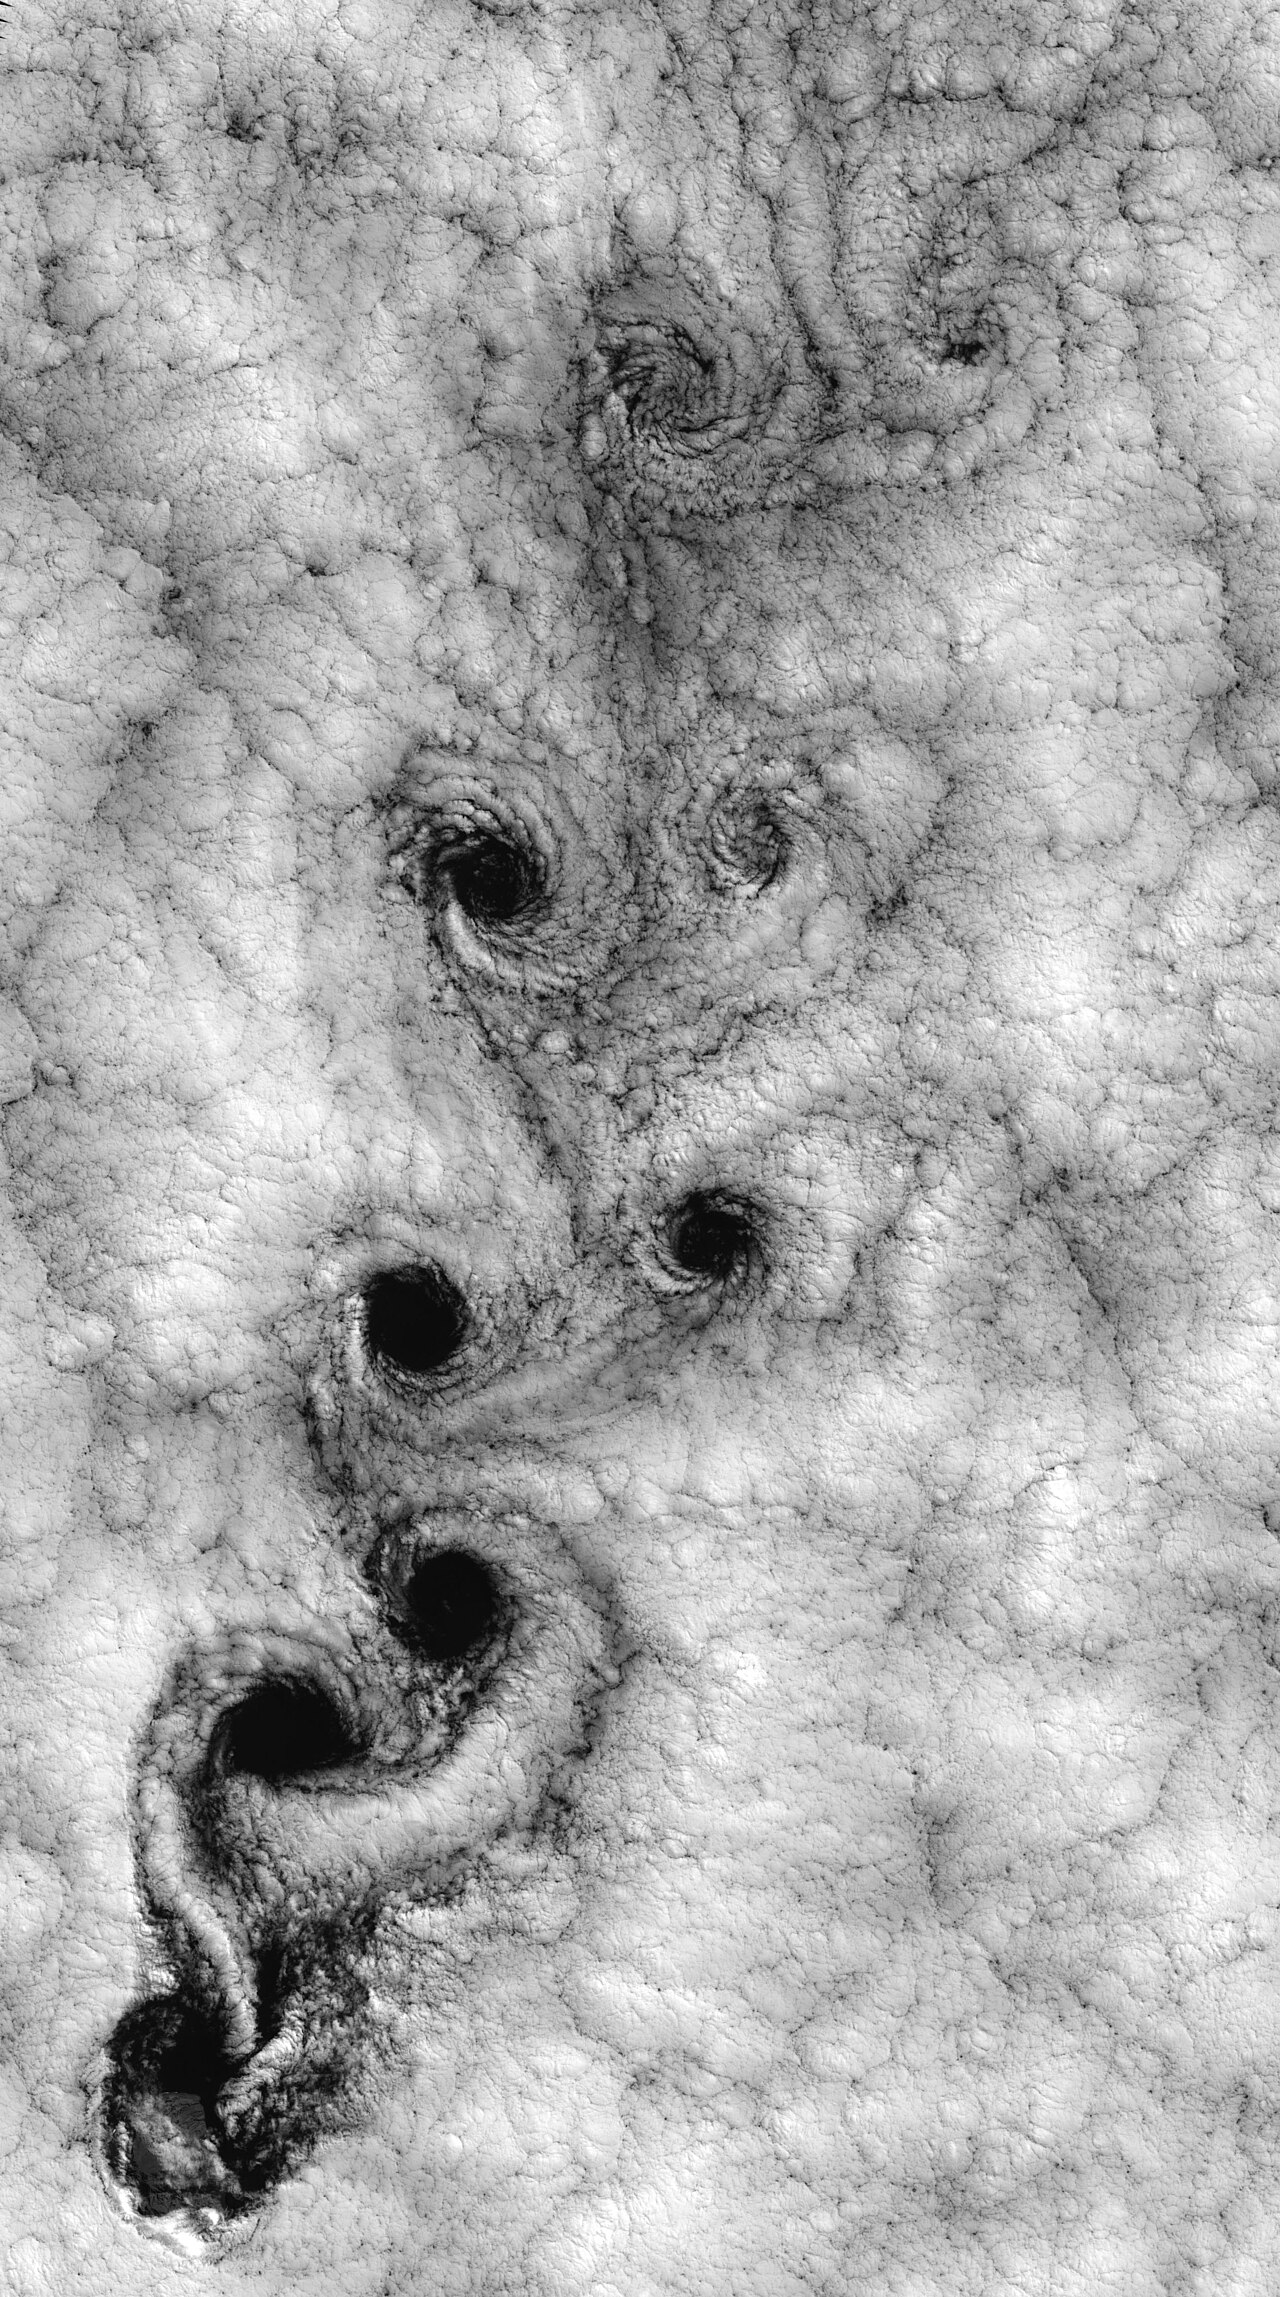
\includegraphics[width=0.34\linewidth]{images/book4/karman-vortex-street.jpg}

{\small 冯·卡门涡街：从太空拍摄的岛屿下游云层中的卡门涡街，即圆柱尾流，雷诺数为数百，图中按百千米量级绘制（NASA）。}
\end{omfigure}

\section{问题：血液、原油与雨滴}

\begin{problem}[{周末问题——同样的黏性规律在动脉中、
千公里管道中以及下落的液滴中}]
\label{pb:b2:viscous-flows:1}

\medskip
\noindent\textbf{第一部分——血液。}
血液：$\rho = \qty{1060}{kg/m^3}$，$\eta = \qty{3.5e-3}{Pa.s}$（视为
牛顿流体）；心输出量 $D_V = \qty{5.0}{L/min}$。
\begin{enumerate}
  \item 主动脉，半径 \qty{1.25}{cm}：求平均速率、雷诺数，并判断流动类型。
  \item 若主动脉中的流动为泊肃叶流，其最大速率与
        管壁切应力各为多少？（内皮细胞能感知
        约 \qty{1}{Pa} 量级的应力。）
  \item 毛细血管，半径 \qty{4.0}{\micro m}，血液流速为
        \qty{0.30}{mm/s}：求雷诺数；求其
        \qty{1.0}{mm} 长度上的压强降，分别以帕斯卡和毫米汞柱表示
        （\qty{1}{mmHg} = \qty{133}{Pa}）。
  \item 红细胞穿过毛细血管所需的时间；为何这一
        量级恰好适合气体交换？
  \item 小动脉（半径 \qty{10}{\micro m}，长 \qty{2.0}{mm}，$10^8$
        根并联）：求这组小动脉的总流阻，以及
        在满负荷心输出量下两端的压强降。
  \item 动脉到静脉的总压降为 \qty{13}{kPa}：求左心室输出的
        机械功率，并与
        \qty{100}{W} 的人体相比较。
  \item 一处狭窄使冠状动脉的半径在一小段内减小 $40\%$：
        求其流阻升高的倍数；为何
        静息时下游心肌可能仍能得到供血，
        而在剧烈运动时则不能。
  \item 剧烈运动时心输出量达到 \qty{25}{L/min}：
        求主动脉中的雷诺数，并判断流动类型。
  \item 血液并非牛顿流体：其表观黏度在高剪切速率下降低，
        在低剪切速率下升高。上述血管中哪一种受影响最大，
        且变化方向如何？
\end{enumerate}

\medskip
\noindent\textbf{第二部分——管道。}
一条原油输送管道：直径 $D = \qty{1.2}{m}$，长度 $L = \qty{1300}{km}$，
流量 $D_V = \qty{3.0}{m^3/s}$；原油 $\rho = \qty{850}{kg/m^3}$，$\eta =
\qty{2.0e-2}{Pa.s}$（保温时）。湍流摩擦规律：$\Delta P = \lambda
(L/D)\tfrac12\rho\langle v\rangle^2$, $\lambda = 0.316/\mathrm{Re}^{1/4}$.
\begin{enumerate}[resume]
  \item 求平均速率与雷诺数，并判断流动类型。
  \item 求每千米的压强降，以及整条管线的压强降。
  \item 管道能承受 \qty{80}{bar}：求沿线
        所需泵站的最少数目。
  \item 求总泵功率；求每立方米送达原油所需的能量，
        并与原油的能量含量（\qty{36}{GJ/m^3}）比较。
  \item 按泊肃叶定律，压强降应为多少？评论
        湍流的代价（以及为何某些管线中要注入能延缓
        湍流的聚合物添加剂）。
  \item 冬季未加热的原油黏度将达到 $\eta = \qty{2.0}{Pa.s}$：
        求新的雷诺数与流动类型；用相应的规律求整条管线的压强降。
        对设计作出结论（实际管线有保温层，
        原油保持温热）。
  \item 原油从一端输运到另一端所需的时间。
  \item 由压强降求温热、湍流情形下的管壁切应力；
        并求管道壁面受到的总摩擦力。
  \item 同样的流动在 \qty{1.0}{m} 管道中，
        湍流压强降变为原来的多少倍？
  \item 一粒 \qty{0.10}{mm} 的沙粒（$\rho_s = \qty{2650}{kg/m^3}$）随温热的原油输运：
        求斯托克斯沉降速率与沙粒的雷诺数，
        以及沉降穿过管道所需的时间；将其与湍流速度脉动
        （约为 $\langle v
        \rangle$ 的百分之几）相比较：沙粒在运行中的管道内会沉降吗？
        在停止的管道内呢？
\end{enumerate}

\medskip
\noindent\textbf{第三部分——液滴。}
空气：$\rho = \qty{1.2}{kg/m^3}$，$\eta = \qty{1.8e-5}{Pa.s}$；水 $\rho_w =
\qty{1000}{kg/m^3}$, $\gamma = \qty{0.072}{N/m}$.
\begin{enumerate}[resume]
  \item 云滴，直径 \qty{10}{\micro m}：求斯托克斯终端速度、
        雷诺数，以及下落 \qty{1}{km} 所需的时间；为何云能悬浮不落。
  \item 毛毛雨，直径 \qty{0.20}{mm}：求斯托克斯速率与雷诺数；
        斯托克斯公式是否仍然可靠？
  \item 雨滴，直径 \qty{2.0}{mm}：证明斯托克斯公式不再适用，并求
        终端速度（取 $C_x = 0.5$），以及从 \qty{1}{km} 高处落下所需的时间。
  \item 在 \qty{1}{cm/s} 的上升气流中，云滴是
        上升还是下落？多大的上升气流能托住毛毛雨滴？
  \item 求三个液滴内部的拉普拉斯压强，并分别与
        动压 $\tfrac12\rho v_\infty^2$ 比较，解释为何大雨滴在
        直径超过约 \qty{5}{mm} 时会压扁并破碎。
  \item 用一张表格给出本题中八种流动的
        雷诺数及支配其运动的规律。
\end{enumerate}
\end{problem}
